\documentclass[t]{beamer}
%\usetheme{iclpt}
\usepackage{url}
\usepackage{pifont}
\usepackage{amscd}
\usepackage{MnSymbol}
\newcommand{\tick}{{\color{green}\ding{51}}}
\newcommand{\dcross}{{\color{red}\ding{55}$\,$}}
\usepackage{pythonhighlight}
\newcommand{\dd}[2]{\frac{\diff#1}{\diff #2}} 
\def\MM#1{\boldsymbol{#1}}
\beamertemplatenavigationsymbolsempty
\author[Colin Cotter]{Prof. Colin Cotter}
\institute{Imperial College London}
\DeclareMathOperator{\diff}{d\!}
\DeclareMathOperator{\Div}{div}
\DeclareMathOperator{\Id}{Id}
\DeclareMathOperator{\Ro}{Ro}
\DeclareMathOperator{\ccurl}{curl}
\DeclareMathOperator{\ddiv}{div}
\DeclareMathOperator{\Tr}{Tr}
\newcommand{\pp}[2]{\frac{\partial #1}{\partial #2}} 
\newcommand{\Hcurl}{H(\operatorname{curl})}
\newcommand{\Hdiv}{H(\operatorname{div})}
\newcommand{\comment}[1]{}
\newcommand{\jump}[1]{\left[\!\left[ #1 \right]\!\right]}
\title[CCMI]{EPSRC Centre for Doctoral Training in
  Collaborative Computational Modelling at the Interface\\
  \vspace{5mm}
  
\includegraphics[width=4cm]{ccmi_square_colour_text}
  \hspace{5mm}
  
\includegraphics[width=4cm]{ukri_logo}}

\newtheorem{proposition}[theorem]{Proposition}
\newcommand{\dede}[2]{\frac{\delta #1}{\delta #2}}
\newenvironment{packed_enum}{
\begin{enumerate}
  \setlength{\itemsep}{1pt}
  \setlength{\parskip}{0pt}
  \setlength{\parsep}{0pt}
}{\end{enumerate}}

\newcommand{\V}{\mathbf{V}}
\newcommand{\U}{\mathbf{U}}
\newcommand{\W}{\mathbf{W}}
\newcommand{\M}{\mathrm{M}}
\newcommand{\R}{\mathrm{R}}
\newcommand{\La}{\mathrm{L}}
\newcommand{\Fu}{\mathbf{F}}


\usepackage{tikz}
\usepackage{amsmath}
\usetikzlibrary{trees,positioning}

\newenvironment{packed_item}{
\begin{itemize}
  \setlength{\itemsep}{1pt}
  \setlength{\parskip}{0pt}
  \setlength{\parsep}{0pt}
}{\end{itemize}}

\begin{document}

\date{July 17th 2024}

\frame{\maketitle}

\frame{
  \vfill
  \frametitle{What is CCMI about?}
  \begin{block}{}
  CCMI is a collaboration between University College London and
  Imperial College London to offer a novel and innovative PhD training
  programme at the interface of computational modelling, data
  sciences, and research software engineering.
  \end{block}
  Key participating departments:
  \begin{itemize}
  \item Imperial Mathematics
  \item Imperial Computing
  \item UCL Advanced Research Computing Centre
  \item UCL Mathematics
  \item UCL Statistics
  \item UCL Computing
  \end{itemize}
\vfill
}

\frame{
  \frametitle{Partners}
  \begin{itemize}
  \item Imperial and UCL
  \item UKAEA
  \item Crick Institute
  \item GAMS,FICO, DataSparq, SLB, McLaren Racing, Graphcore, DELL,
    ATI, BASF, Gurobi, SURF, Enthought, Rapiscan, Rafinex ...
  \end{itemize}
}

\frame{
  \frametitle{Training focus}
  \vfill
  What do we research?
  \begin{itemize}
  \item Computational models based on physical principles, or
    constructed from data, or both.
  \item Spanning from reduced modelling to high performance computing.
  \item Modelling applications in: engineering, nuclear fusion,
    medicine and systems biology, weather and climate, imaging science,
    ecology, finance, and beyond.
  \item Algorithms for solving problems using models: data assimilation,
    optimisation, control and decision making.
  \end{itemize}
  \vfill
}

\frame{
  \frametitle{Research priorities}
  \vfill
  \begin{itemize}
  \item \structure{Mathematical foundations}: we seek to quantify
    stability, accuracy, approximation, model reduction, complexity,
    bifurcation phenomena, etc for hybrid models, and use these ideas
    to build efficient discretisations and fast numerical solvers
    for them.
  \item \structure{Computational algorithms}: the enrichment of
    classical scientific computing algorithms with data, aiming to
    reach grand challenge applications where algorithms would otherwise
    fail.
  \item \structure{Scientific research software engineering}: the
    ability to reliably, scalably and maintainably realize complex
    mathematically sophisticated and data intensive solutions as code
    is fundamental to the challenge.
  \item \structure{Bridging the gap to applications}: translation to
    applications science, facilitated by our broad range of
    applications cosupervisors and project partners, who are working
    with computational models across science and engineering.
  \end{itemize}
  \vfill
}

\frame{
  \vfill
  \centerline{
  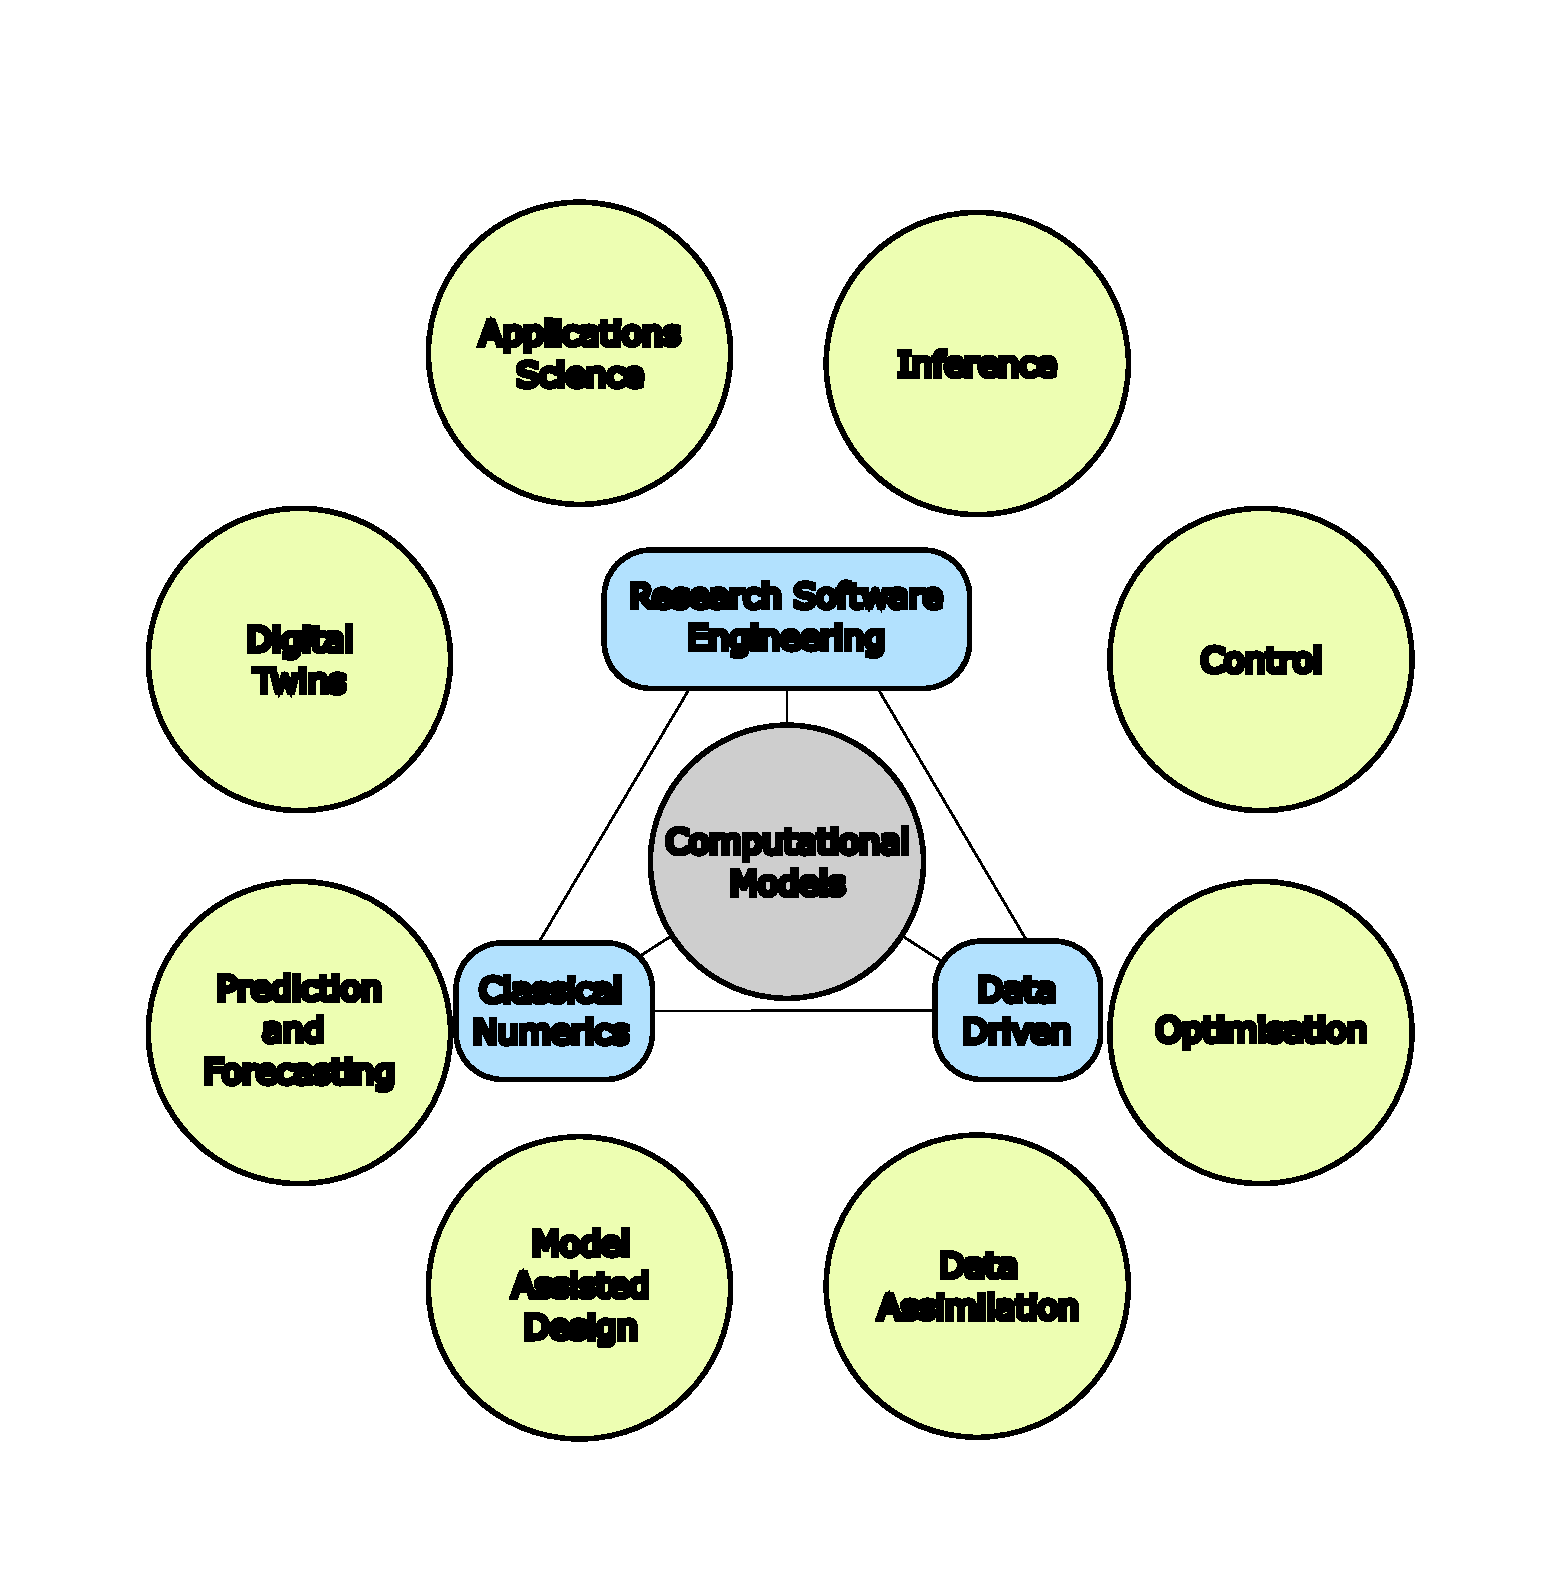
\includegraphics[width=9cm]{CDTcircle}}
  \vfill
}

\frame{
  \frametitle{What do we train?}
  \vfill
  \begin{enumerate}
  \item A four year research thesis on the interface of computational
    sciences, research software engineering, and data sciences.
  \item
    Collaborative interface working groups: week long block events
    that combine topical overviews, research discussions, software
    exploration, and discovery of new ideas.
  \item Software journey: involves active collaboration in
    open-source projects, close collaboration with external
    partners, regular software weeks, sprint sessions, industry
    talks on software engineering, and many other activities.
  \end{enumerate}
  \vfill
}

\frame{ \vfill \centerline{ 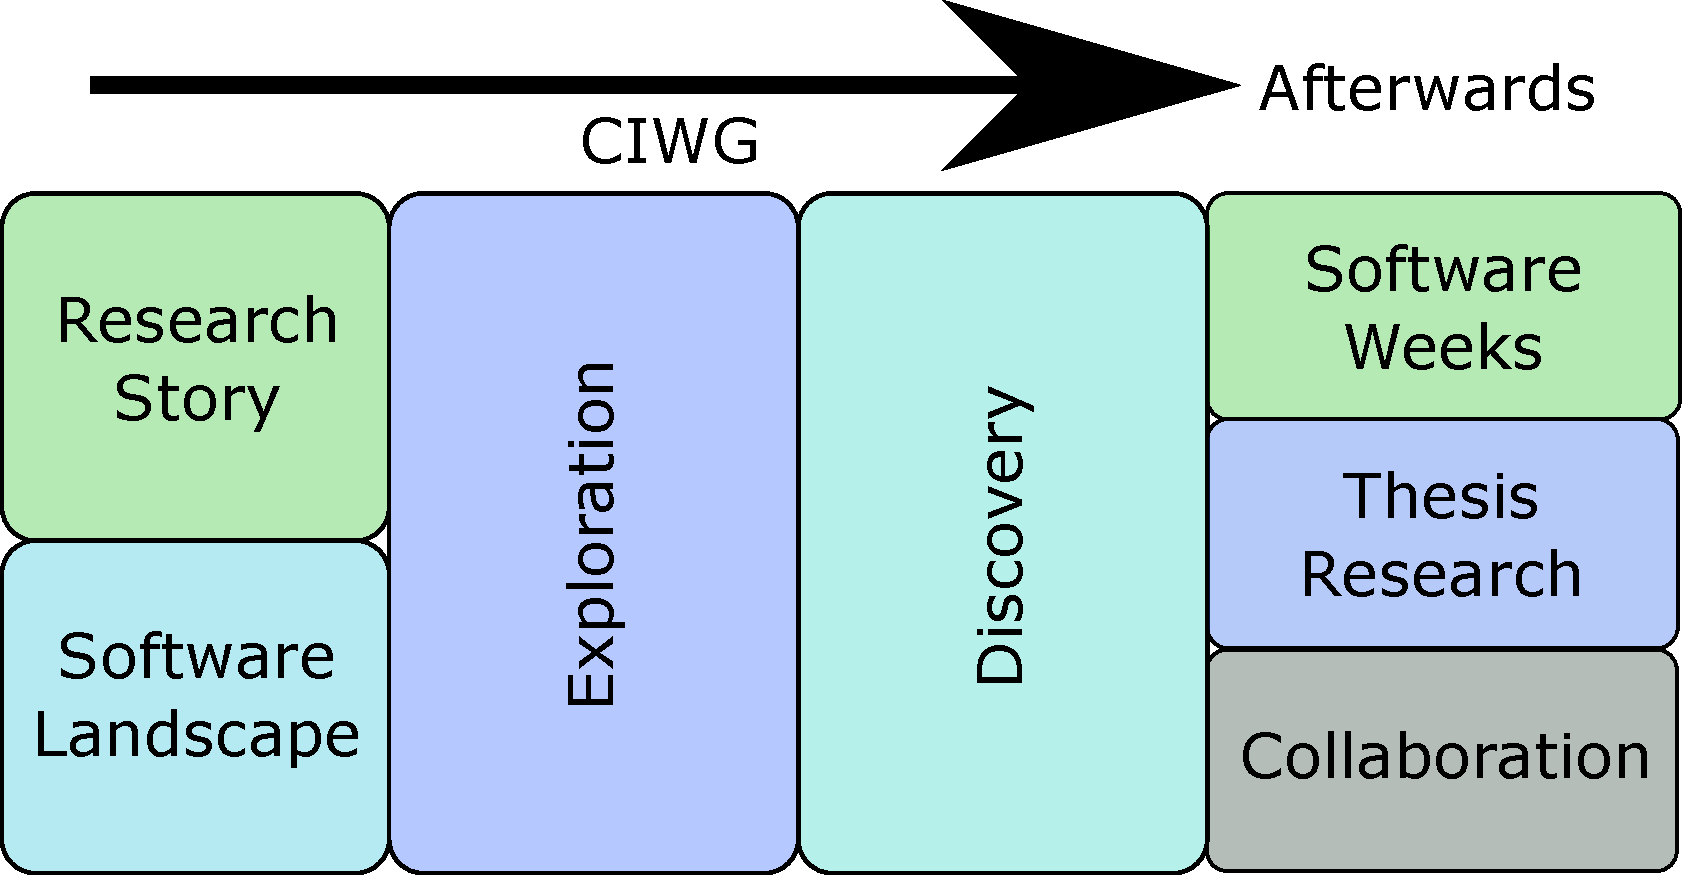
\includegraphics[width=9cm]{cwig}} \vfill
  Example topics: Modern programming models for scientific computing,
  Data intensive computations, Deep learning in theory and practice,
  High dimensional problems and optimisation.  }
  
\frame{
  \vfill
  \centerline{
    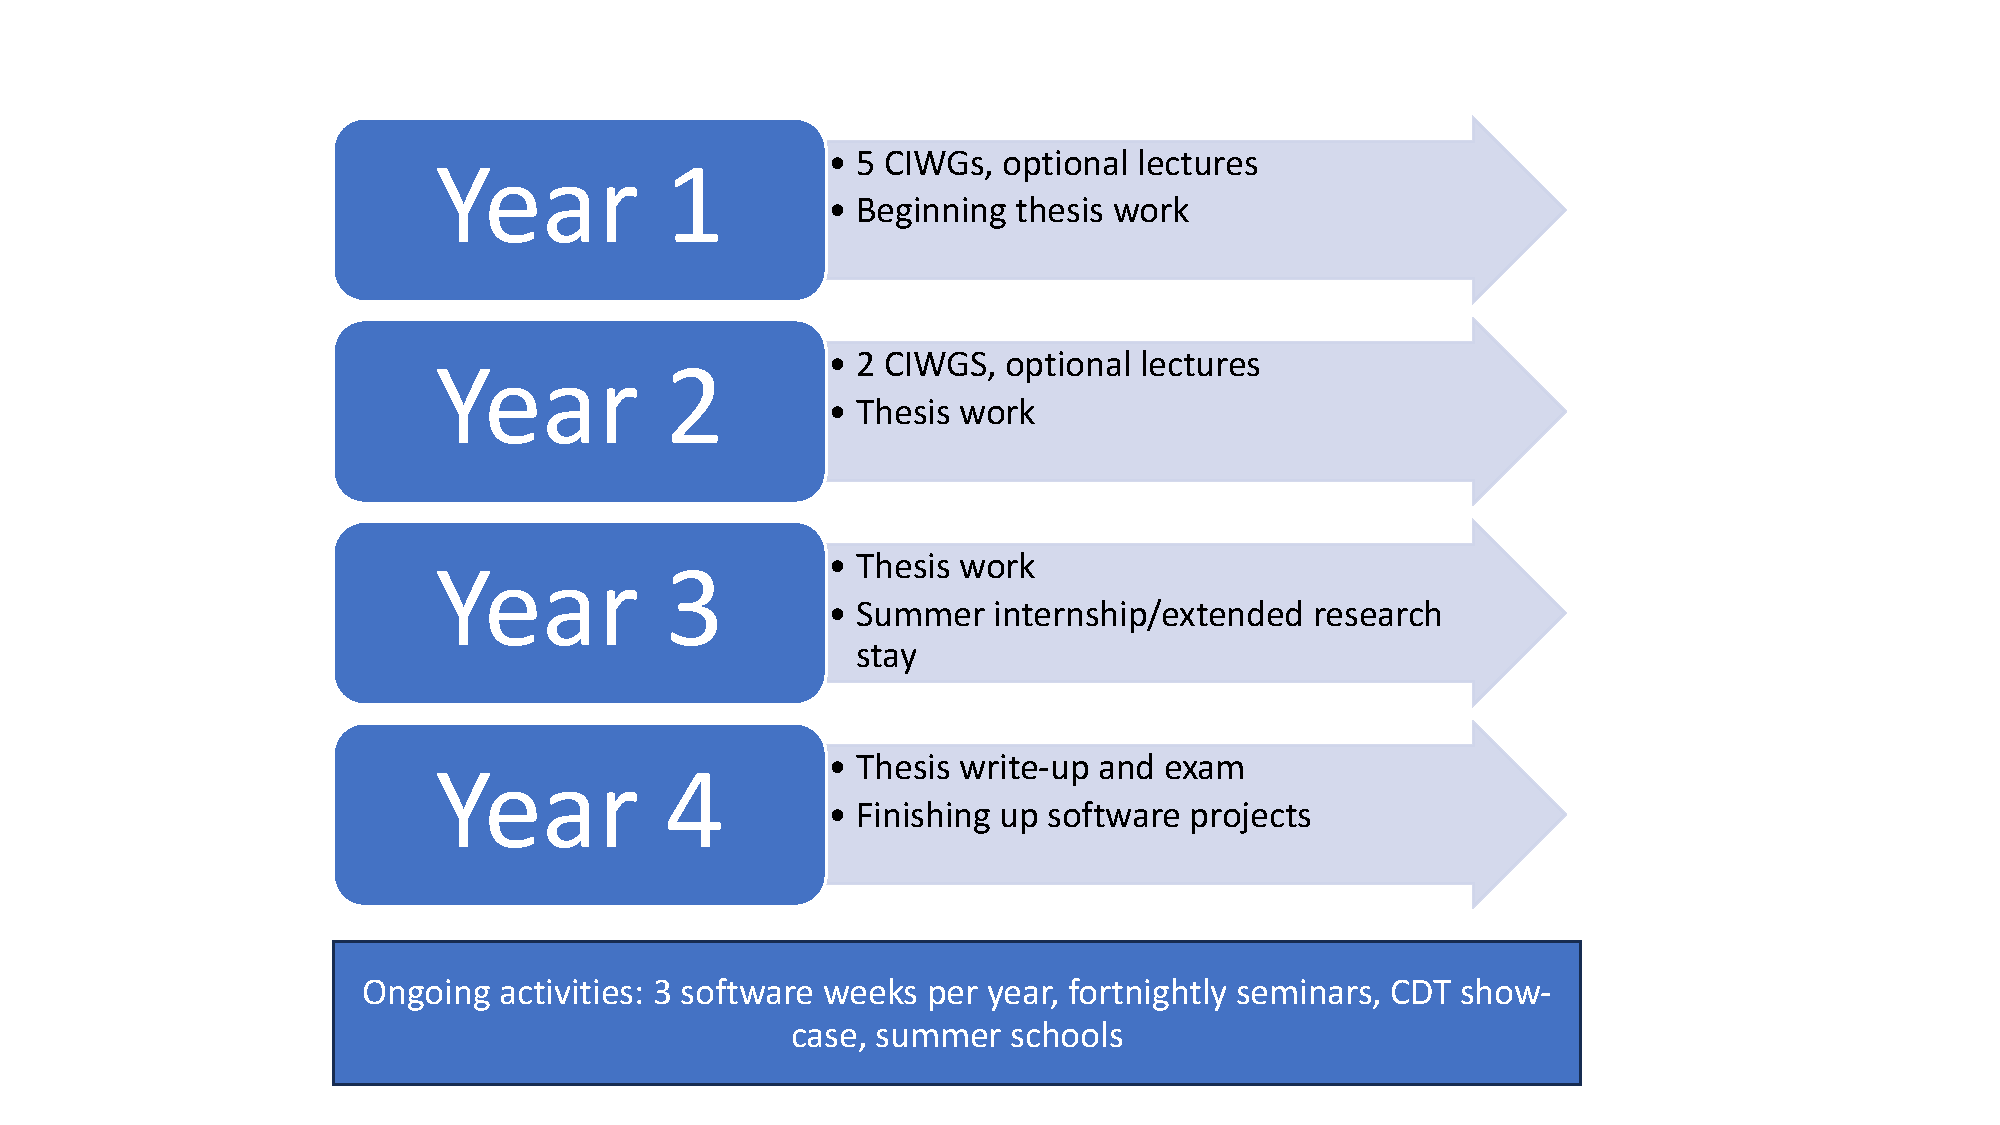
\includegraphics[width=9cm]{CDTFlow}}
  \vfill
}

\frame{
  \frametitle{The team}
  \begin{center}
    \includegraphics[height=2.5cm]{betcke}
    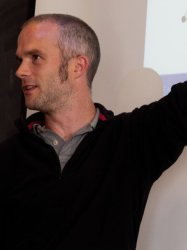
\includegraphics[height=2.5cm]{cotter}
    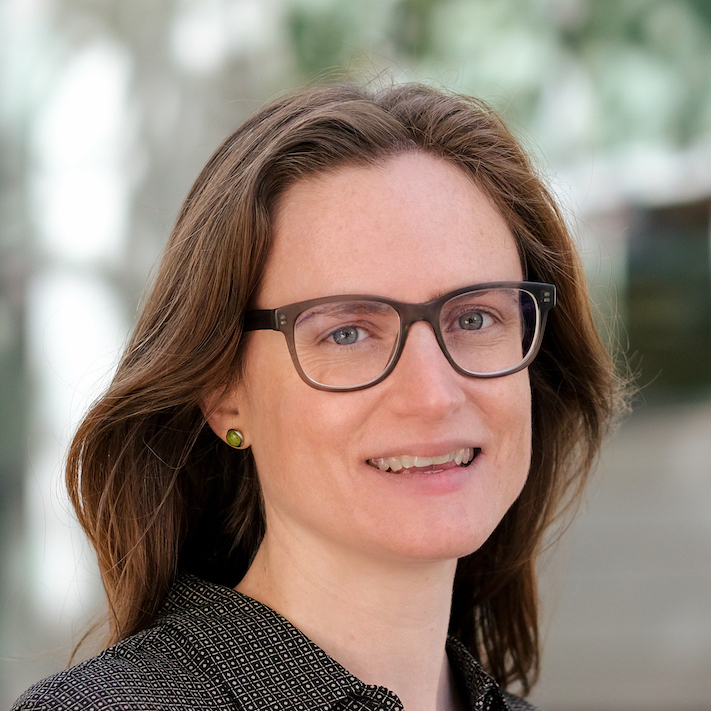
\includegraphics[height=2.5cm]{misener}
    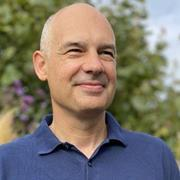
\includegraphics[height=2.5cm]{guillas}\\
    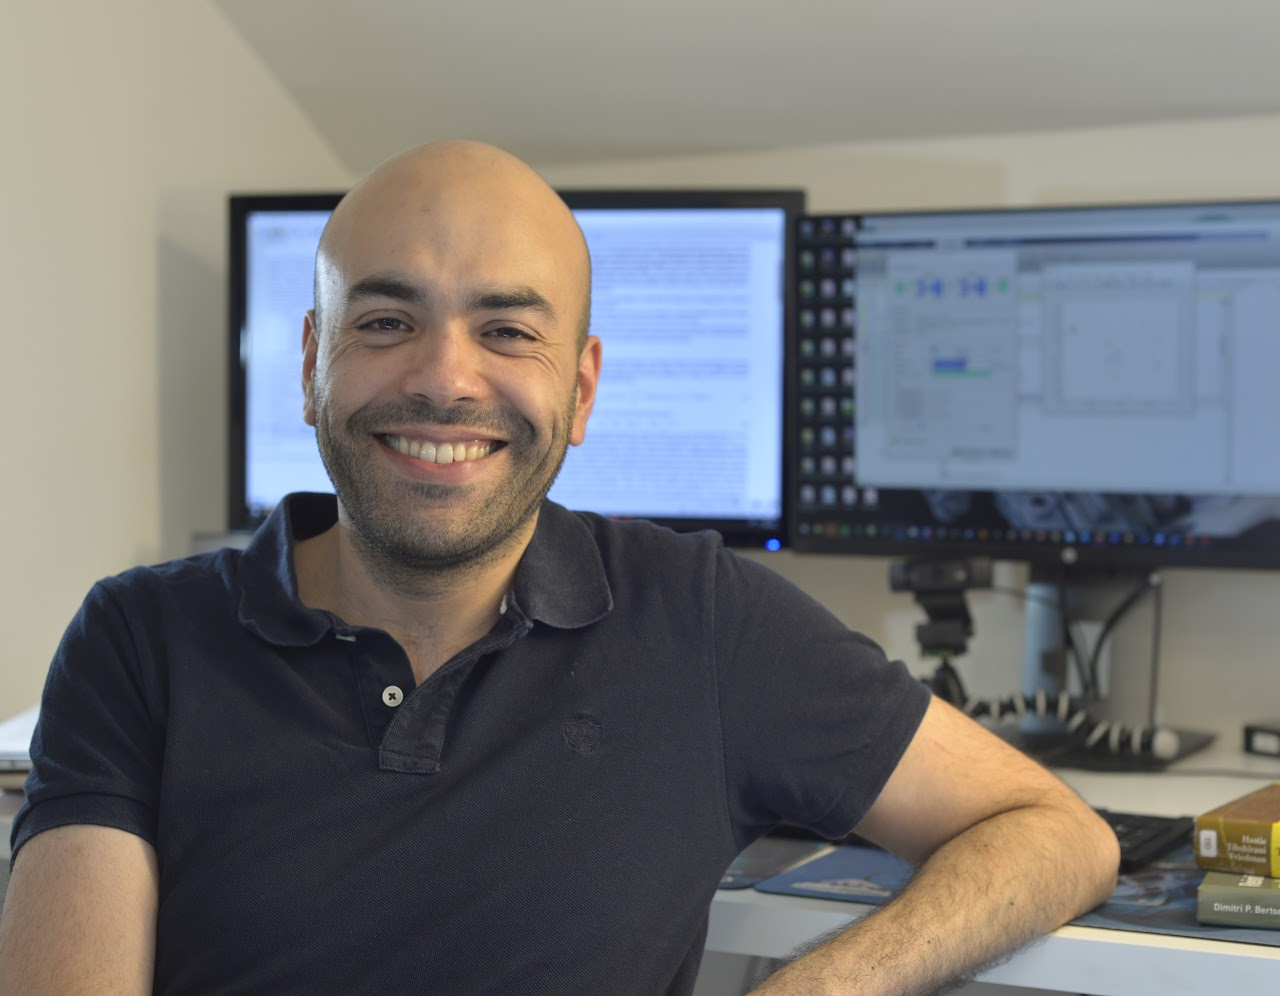
\includegraphics[height=2.5cm]{kalise}
    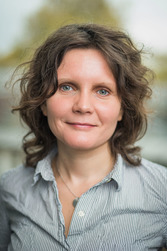
\includegraphics[height=2.5cm]{mbetcke}
    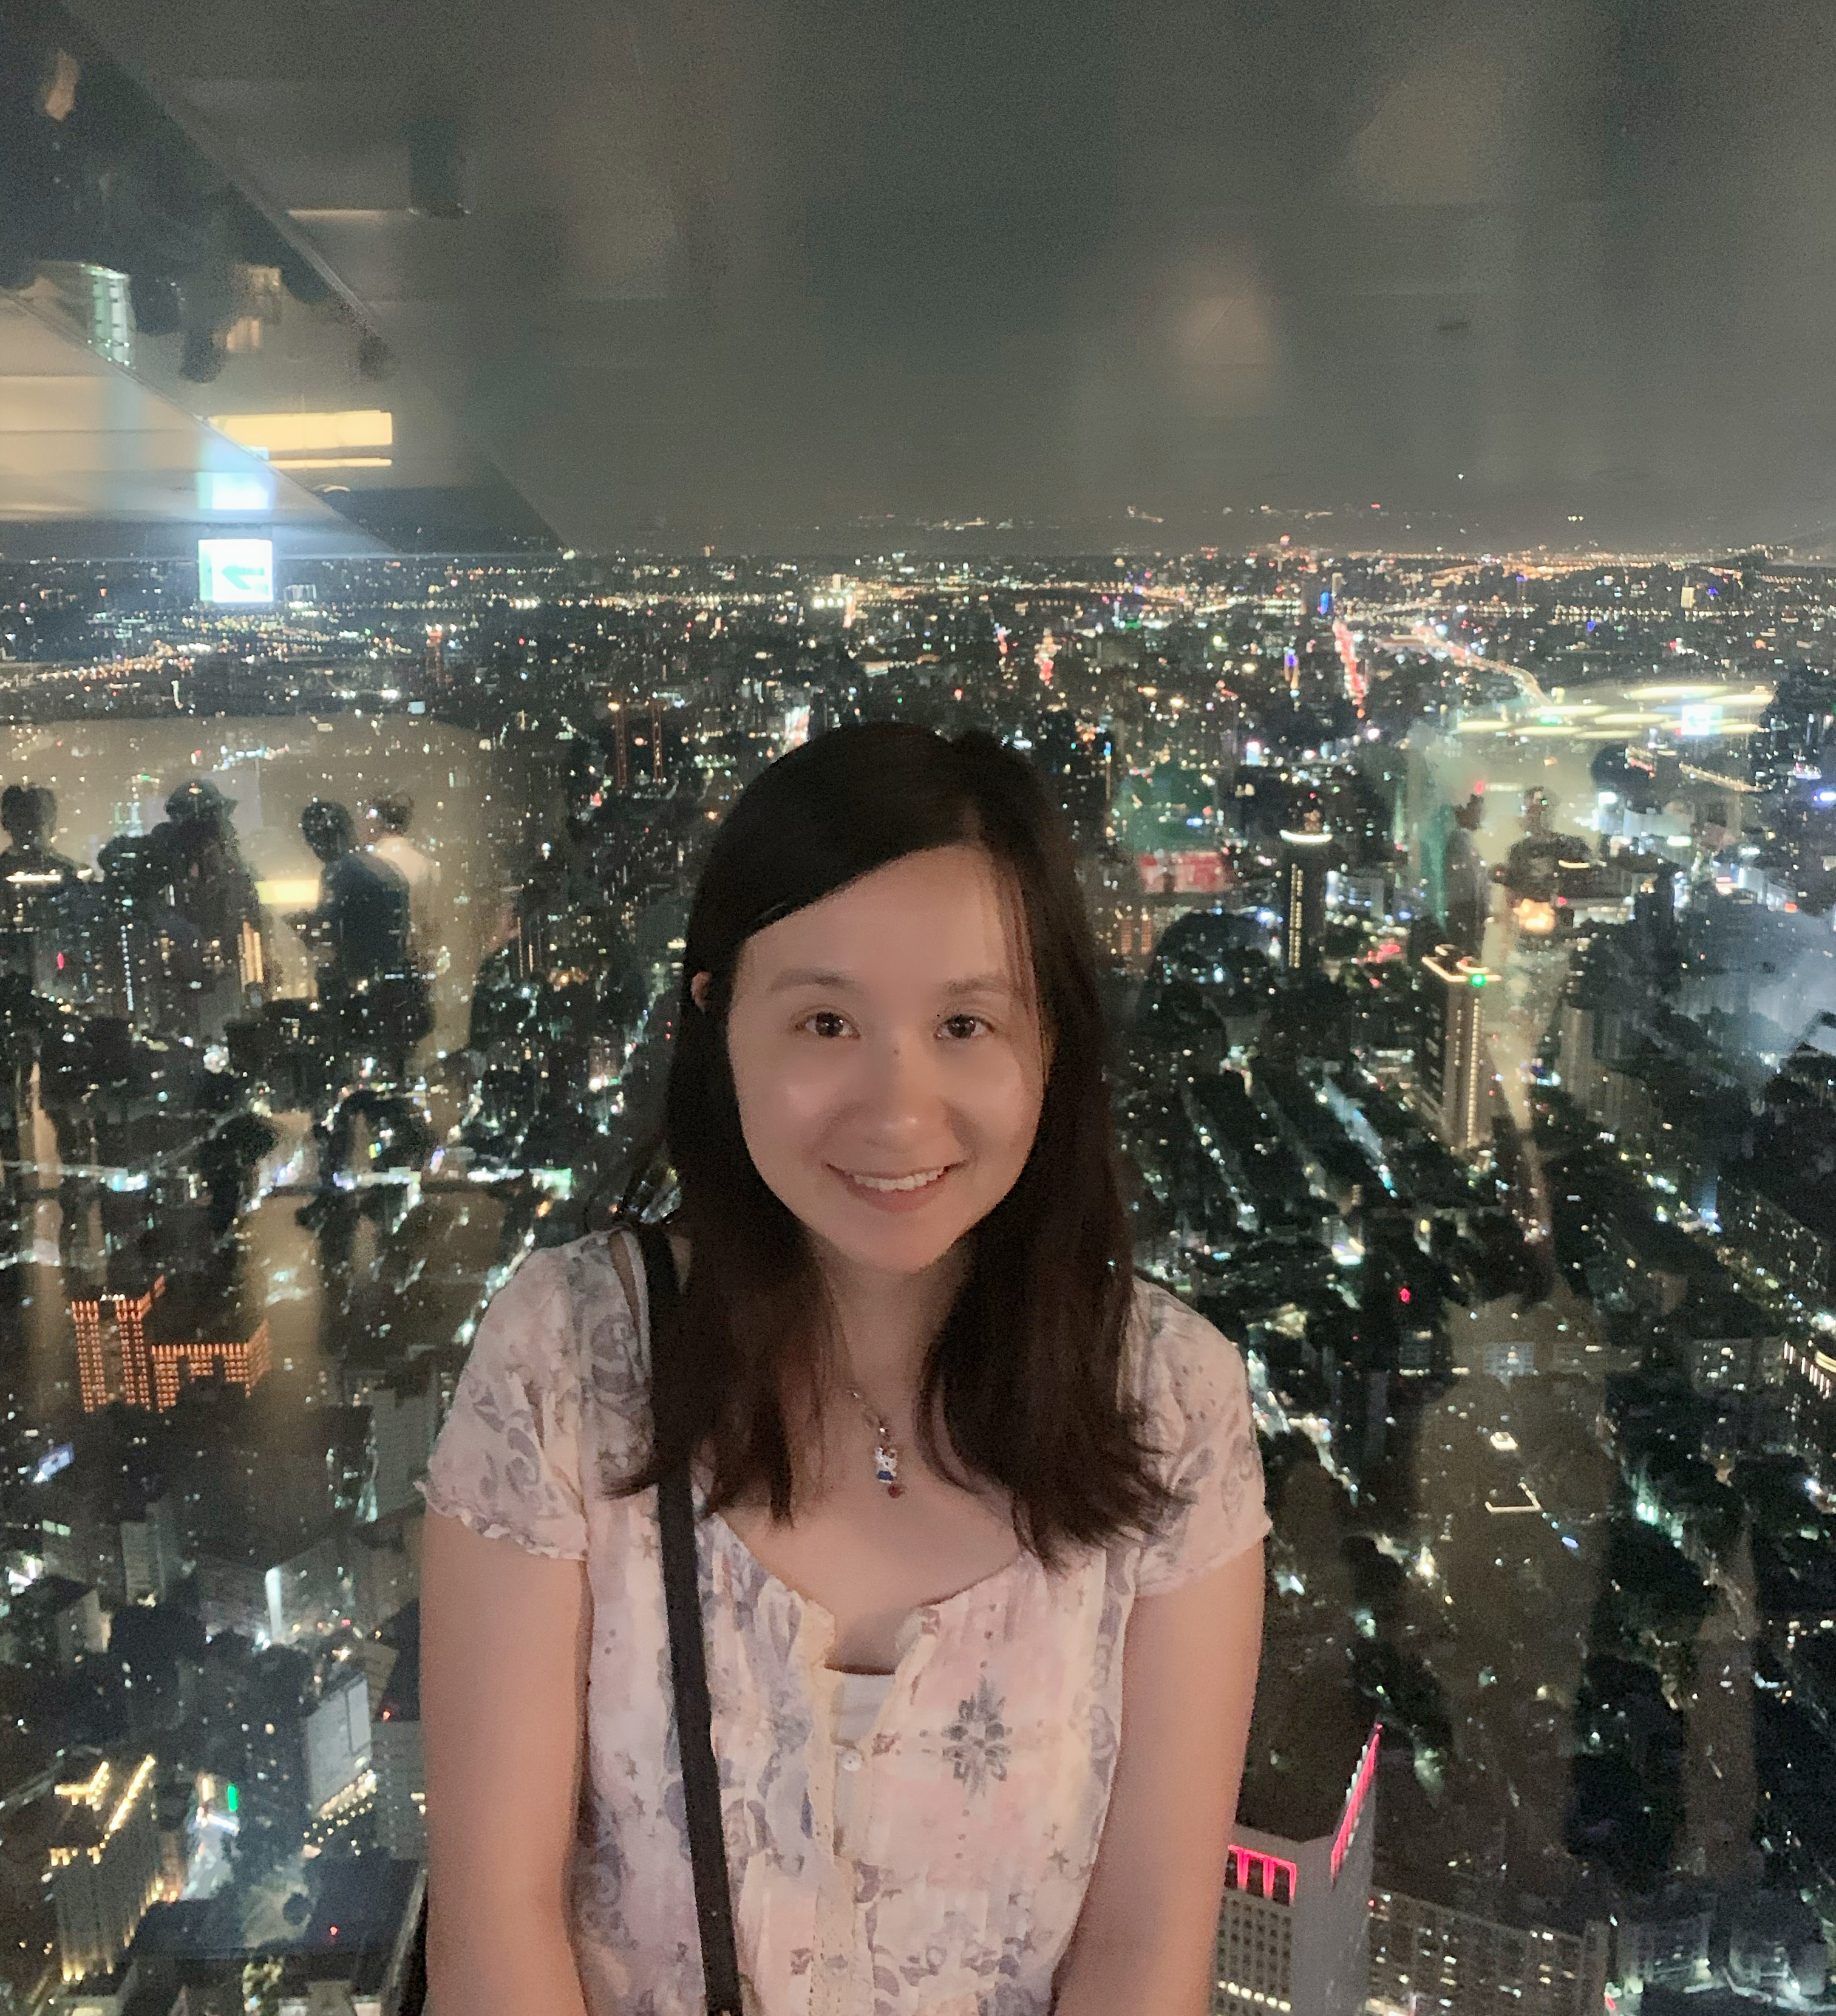
\includegraphics[height=2.5cm]{ni}
    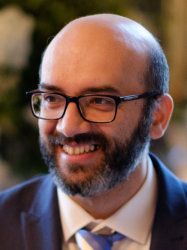
\includegraphics[height=2.5cm]{shahrezaei}
  \end{center}
  Timo Betcke, Colin Cotter, Ruth Misener, Serge Guillas \\
  Dante Kalise, Marta Betcke, Ni Hao, Vahid Sharezaei
}

\frame{
  \frametitle{Is it you?}
  We are looking for future PhD researchers who:
  \begin{itemize}
  \item have the ambition to build and understand cutting edge computer
    models
  \item are curious about algorithms that combine physical laws and
    information from measured data
  \item want to do research driven by what is possible with excellent
    software practices
  \item want to change the world for the better using computational modelling
  \end{itemize}
  \vfill
  Questions?
}

\end{document}
